\chapter{Exploratory Study}

\section{Motivation}
What was the purpose of the study?
What were the hypotheses?

\section{Dataset}
What was the dataset?


How did you get the dataset?
 

Why those sources?
 


% What’s CrowdFlower?
 
% What’s the difference between CrowdFlower and Turk?
 

% How did you control for quality?

% CrowdFlower has a built-in “Test Question” feature that allows for the rejection of a annotator whose answers to specific questions do not lie within a threshold (default 70%) of the “correct” answer or whose answers lay outside the standard variation compared to others.

% However, since the questions we asked were by nature subjective and therefore outliers and disagreements in answers could imply signal rather than noise, we chose to monitor for quality using other metrics instead. CrowdFlower was not designed explicitly for survey-like tasks, and therefore there were no options for different screening methods or questions. Gold Questions on the platform are selected by the creator within the set of all questions being recorded.

% Because of this, we monitored quality of results in two ways:

% First, by setting a minimum of time of 180 seconds to complete the task of reading 5 stories for a task to be accepted,

% And second, by selecting only Level 3 workers on CrowdFlower as suggested on their website for handling survey-like tasks.
% [https://success.crowdflower.com/hc/en-us/articles/201855969-Survey-Guide-To-Running-Surveys] 

% Users were also only allowed to answer the set of questions once. 

% Average response time was 07:31 minutes.
 

 
% What kind of people signed up for your study?

 
% What was the duration, n size, etc.
 

% How did you recruit them? What was their incentive?
 

% What kind of effects were you looking for?
 
% What kind of effects did you find?

% Trustworthiness

% How do your trustworthiness findings line up with the findings from Pew surveys?

% What about favorability?
  




  


% Basic stats here:
% we ran over X days
% over data points

% \section{Reader Demographics}

% \section{Media Favorability of Candidates}
% Each reader was asked to score the five stories according to how favorable each one was to the featured candidate (by headline). 

% \begin{figure}[h!] 
% \centering
%   \fbox{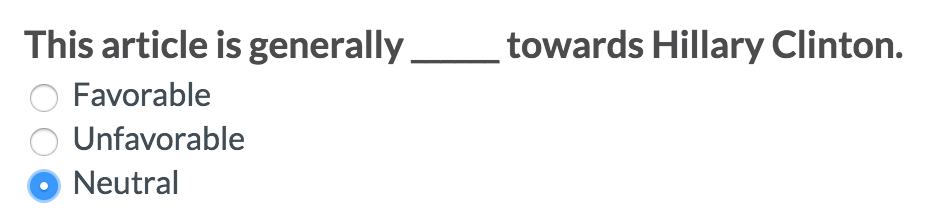
\includegraphics[width=0.5\textwidth]{favorability_question}}
%   \caption{Example of favorability scoring question}
% \end{figure}
 
% Scores were collected on a three-point scale, Favorable (1), Unfavorable (-1), or Neutral (0).

% Overall, media coverage of Trump was viewed as most negatively biased, with over half of stories (51.1\%) viewed as unfavorable towards the candidate.

% Of the stories shown, both Sanders and Clinton were viewed as having more positive than negative coverage, at 38.9\% of the 180 annotations being positive. Sanders also had the least negative coverage, with only 18.3\% stories shown being viewed as negatively biased against the candidate. Republican candidate Cruz was also seen to have more negative (33.3\%) than positive (28.9\%) stories about him, although the majority were seen as neutral (37.8\%).

% \begin{figure}[h!] 
% \centering
%   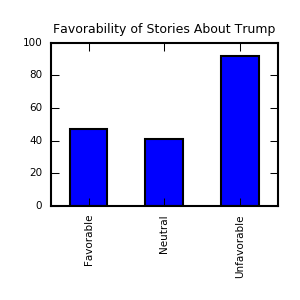
\includegraphics[width=0.45\textwidth]{Trump_favorability} 
%   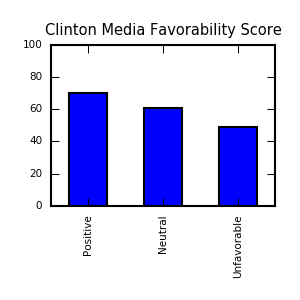
\includegraphics[width=0.45\textwidth]{Clinton_favorability} 
%   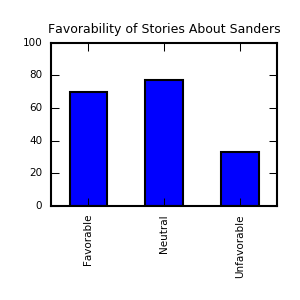
\includegraphics[width=0.45\textwidth]{Sanders_favorability} 
%   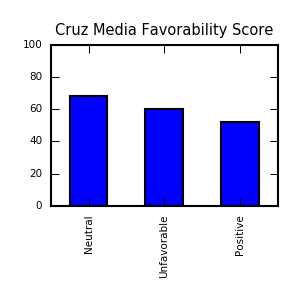
\includegraphics[width=0.45\textwidth]{Cruz_favorability} 
%   \caption{Media Favorability of Candidates}
% \end{figure}

% These trends persist when we filter responses by stories that were considered trustworthy or at least neutral (score > 0).

% \begin{figure}[h!] 
% \centering
%   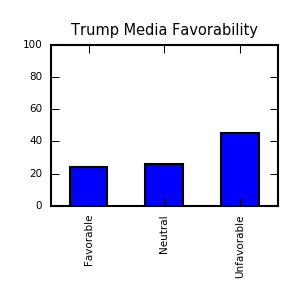
\includegraphics[width=0.45\textwidth]{Trump_favorability_trust_gt_0} 
%   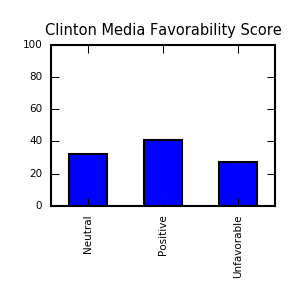
\includegraphics[width=0.45\textwidth]{Clinton_favorability_trust_gt_0} 
%   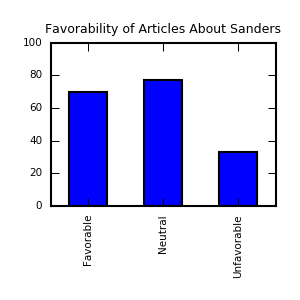
\includegraphics[width=0.45\textwidth]{Sanders_favorability_trust_gt_0} 
%   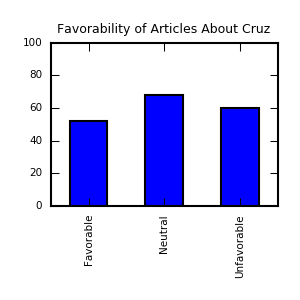
\includegraphics[width=0.45\textwidth]{Cruz_favorability_trust_gt_0} 
%   \caption{Media Favorability of Candidates, Trustworthy Articles}
% \end{figure}

% In the following section, we examine more patterns of media trustworthiness.


% \section{Media Trustworthiness}

% Each reader was also asked to score the five stories according to how trustworthy they found each to be. 

% \begin{figure}[h!] 
% \centering
%   \fbox{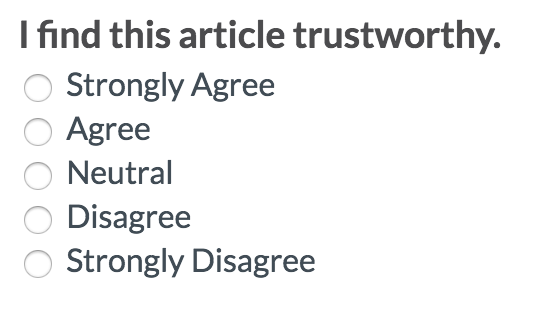
\includegraphics[width=0.35\textwidth]{trustworthy_question}}
%   \caption{Example of trustworthiness scoring question}
% \end{figure}

% Scores were collected on a five-point (Likert) scale: Strongly Agree (2), Agree (1), Neutral (0), Disagree (-1), Strongly Disagree (-2). Overall, readers seldom slected ``Strongly Disagree'', and the option consisted of less than 2\% of all choices.

% In the analysis below, we collapse the results into three categories: Agree (> 0), Neutral (0), and Disagree (<0).

% Despite reportings on national distrust of news, the majority of stories were marked as trustworthy for all candidates.

% \begin{figure}[h!] 
% \centering
%   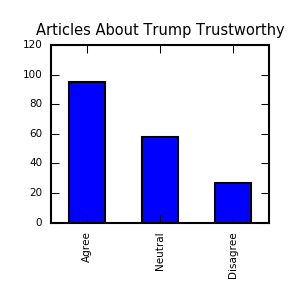
\includegraphics[width=0.45\textwidth]{Trump_trustworthiness_binary} 
%   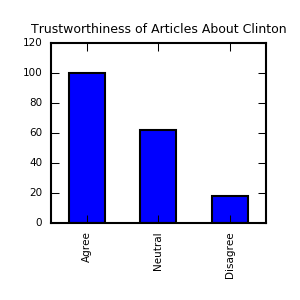
\includegraphics[width=0.45\textwidth]{Clinton_trustworthiness_binary} 
%   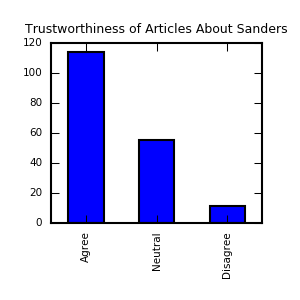
\includegraphics[width=0.45\textwidth]{Sanders_trustworthiness_binary} 
%   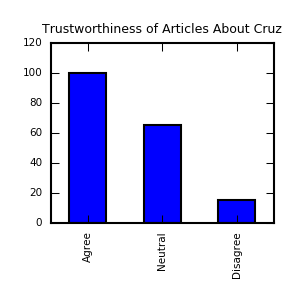
\includegraphics[width=0.45\textwidth]{Cruz_trustworthiness_binary} 
%   \caption{Media Trustworthiness of Candidate Coverage}
% \end{figure}

%  Sanders has strongest trustworthiness, most favorable



 

% \section{Overall Bias Reportings}


% \section{Media Brand Effect}

% \section{Reading Level Effect}

% \section{Other Linguistic Cues}

\section{Limitations}

From our exploratory study, we were able to obtain a significant but weak effect between disclosing the source and the levels of trust marked by readers towards an article.

We also observed trends that suggested an interaction between disclosing the source and the reading level of a story.

However, the study faced several limitations: first, we did not obtain enough samples to show a statistically significant result for interactions between source and reading level.

Furthermore, multiple levels of independent variables (ie: 5 levels for input source) made modeling complex and the results less clear.

The dataset was also unbalanced and sparse (ie, because of large numbers of input variables we did not have complete representation for each category, such as high, low, and mid-reading level stories for every outlet and topic). We tried to control for those factors by randomization, however it made more difficult to analyze specific correlations between source and trust.

To further explore the interaction between disclosing the source and the reading level of the story, we set up another crowdsourcing experiment on CrowdFlower, this time targeting this specific interaction, to see if there is a significant effect between the two, detailed in the following chapter.

% % This is an example of how you would use tgrind to include an example
% % of source code; it is commented out in this template since the code
% % example file does not exist.  To use it, you need to remove the '%' on the
% % beginning of the line, and insert your own information in the call.
% %
% %\tagrind[htbp]{code/pmn.s.tex}{Post Multiply Normalization}{opt:pmn}
%  